\documentclass[12pt,a4paper]{article}
\usepackage[parfill]{parskip}
\usepackage{fullpage}
\usepackage{enumitem}
\usepackage{hyperref}
\usepackage{graphicx}
\usepackage{subfig}

\begin{document}

\vfil

\begin{center}
	{\Large Mobile Robot Systems} \\
	\vspace{0.4in}
	{\huge \bf Assignment 1 } \\
	\vspace{0.4in}
	{\large Anik Roy} \\
	\vspace{0.1in}
	{\large \today} \\
\end{center}
\vspace{0.4in}

% Main document

\section*{1.1 Dynamical Systems and Motion Control}
\subsection*{Exercise 1}
\begin{enumerate}[label=(\alph*)]
	\item $\dot{x} = u\cdot cos(\theta)$\\
	      $\dot{y} = u\cdot sin(\theta)$\\
	      $\omega = cos(t)$
        \item The solution uses Euler's method for approximating the solution to a differential equation. The starting point is decided, then the gradient is computed. A small step (of size dt) is taken along the tangent line computed. The new point is taken as the new starting point, and the procedure continues funcding consecutive points, approximating the curve (which is the solution to the differential equation). In my solution, the poses are the points, where the next pose is calculated by adding the previous pose to the increase in each component. This increase is calculated from the differential equations (which give us the rate of increase of $x$, $y$ and $\theta$). Multiplying the rate of increase by the change in time (dt), gives the amount by which to increase each component to get the next position. This only approximates the position since 
	\item The plot here shows the output of Euler's method with varying step sizes. Smaller step sizes gives a smoother looking curve, since the curve is made up of smaller individual segments. The smaller step size also means that it is closer to the real curve since the tangent lines that euler produces won't go as far away from the real curve.  A smaller step size takes longer to compute, but will produce a solution which is a closer approximation to the real (exact) solution. A larger step size will be quicker to run, but a worse approximation.
	      \begin{figure}[h]
	      	\centering
	      	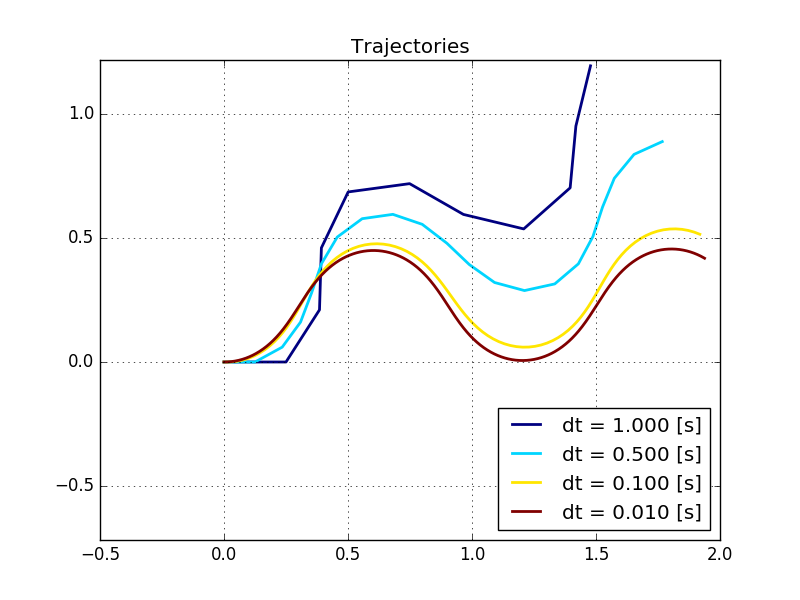
\includegraphics[width=\textwidth]{fig/1c.png}
	      	\caption{Euler's method}
	      	\label{fig:euler}
	      \end{figure}
	\item RK4 is another method for approximating a solution to differential equations. Instead of just using one gradient to calculate a single tangent line, it calculates 4 gradients and combines them to produce subsequent points that are closer to the real curve. In my solution, I calculate the four components that make up the change in theta (one at the start, two halfway across the step size, one at the end of the step) and combine them, weighting them accordingly. I then use these components in calculating the change in $x$ an $y$. Since $\dot{x}$ and $\dot{y}$ are only functions of theta, we need to use these components as arguments to the function.\\
	The equations I used:\\ \\
		  $ \theta_{n+1} = \theta_n + {1\over{6}} (k_1 + 2k_2 + 2k_3 + k_4) $\\
		$k_1 = h\cdot cos(t)$\\
		$k_2 = h\cdot cos(t+h/2)$\\
		$k_3 = h\cdot cos(t+h/2)$\\
		$k_4 = h\cdot cos(t+h)$\\

		$ x_{n+1} = x_n + {1\over{6}} (k_1x + 2k_2x + 2k_3x + k_4x) $\\
		$k_1x = h \cdot u \cdot cos(\theta)$\\
		$k_2x = h \cdot u \cdot cos(\theta+k_1/2)$\\
		$k_3x = h \cdot u \cdot cos(\theta+k_2/2)$\\
		$k_4x = h \cdot u \cdot cos(\theta+k_3)$\\
		
		$ y_{n+1} = y_n + {1\over{6}} (k_1y + 2k_2y + 2k_3y + k_4y) $\\
		$k_1y = h \cdot u \cdot cos(\theta)$\\
		$k_2y = h \cdot u \cdot cos(\theta+k_1/2)$\\
		$k_3y = h \cdot u \cdot cos(\theta+k_2/2)$\\
		$k_4y = h \cdot u \cdot cos(\theta+k_3)$\\
		
	\item Figure \ref{fig:rk4} shows the plot using rk4 instead of Euler. There are several differences between RK4 and Euler. The main one is that Euler is a first order method, and RK4 is a fourth order method, so the error in euler's method decreases on the order of $O(h)$, whereas RK4 is $O(h^4)$, where h is the step size. As the step size gets smaller, the error (difference to exact solution) using RK4 will decrease faster than when using Euler. Euler's method only looks at the single gradient taken at each point to construct a line parallel to the tangent at the curve, whereas RK4 looks at 4 gradients within the step size, and weights them to compute the next point. Taking into account this extra information allows it to converge to the solution quicker. Euler's method can produce acceptable results when the gradient of the curve does not change much, since the error will be smaller. Euler's method is also easier to code and will be quicker to run since it will have to do less calculations. However, it will need a much smaller step size than rk4 so it may not end up being as efficient.
	      \begin{figure}[h]
	      	\centering
	      	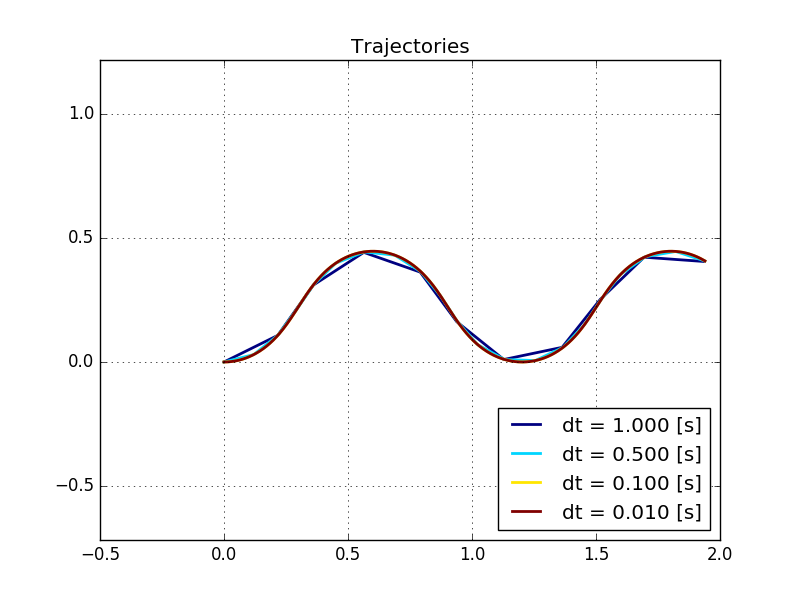
\includegraphics[width=\textwidth]{fig/1e.png}
	      	\caption{RK4}
	      	\label{fig:rk4}
	      \end{figure}
	\item Changing $\omega$ from $cos(t)$ to $cos(\lfloor t \rfloor)$ affects the plots of different step sizes to be closer together.
	      \begin{figure}[h]
	      	\centering
	      	\subfloat[Euler]{{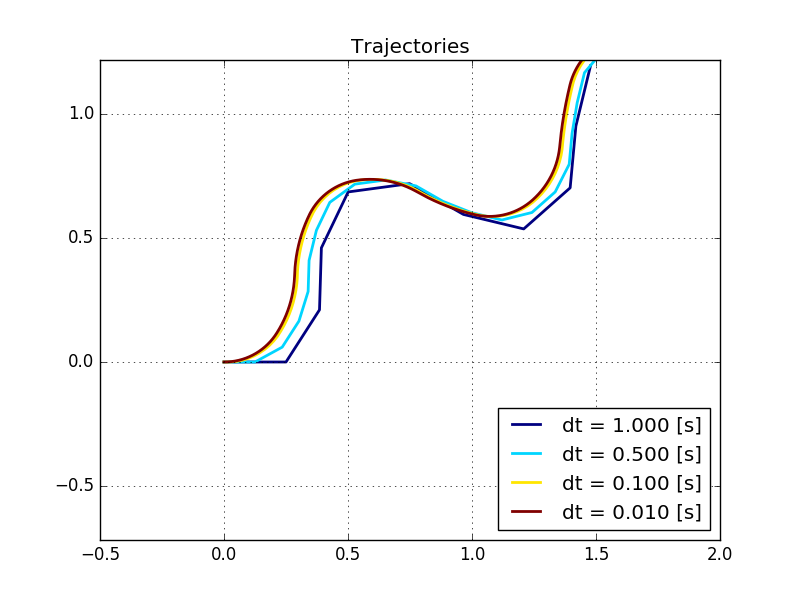
\includegraphics[width=7cm]{fig/1f-euler.png}}}%
	      	\qquad
	      	\subfloat[RK4]{{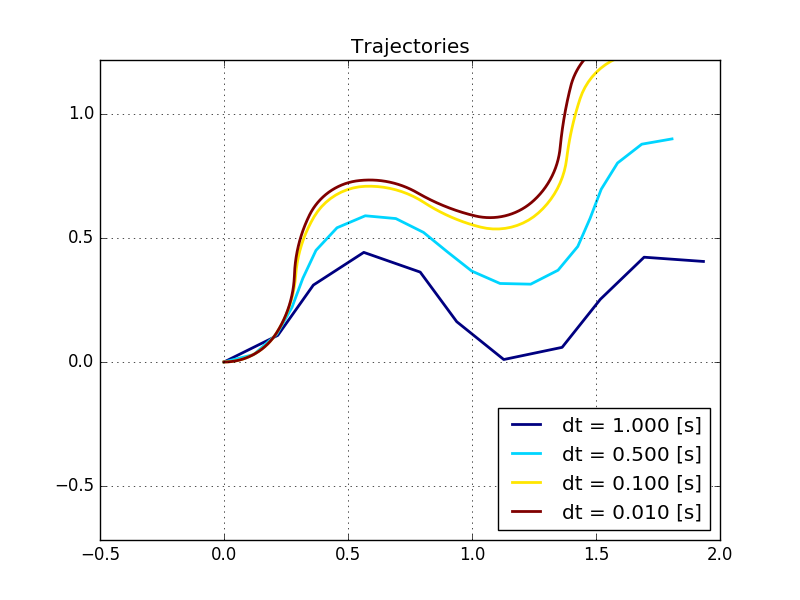
\includegraphics[width=7cm]{fig/1f-rk4-1.png}}}%
	      	\caption{Plots using $\omega=cos(\lfloor t \rfloor)$}%
	      	\label{fig:floor}%
	      \end{figure}
\end{enumerate}
\subsection*{Exercise 2}
\begin{enumerate}[label=(\alph*)]
        \item The plot of my braitenburg controller is shown in Figure \ref{fig:braitenburg}. The velocity decreases as the robot approaches an obstable (according to the log function). The velocity is a function of the front, front\_left and front\_right sensors, with the intuition being that if the robot is close to an obstacle it should decelerate so that it can rotate away from it. For the rotational velocity, this is a function of the front\_left, front\_right, left and right sensors. Since we want to move away from obstacles (the 'coward' example from lecture 4), the rotational velocity will increase (counter-clockwise) if the robot senses it is closer to objects on the right, and vice versa for objects on the left. Both velocities are made up of weighted components of the indivdual sensor values. I estimated and tuned these weights by trial and error.
		\begin{figure}[h]
			\centering
			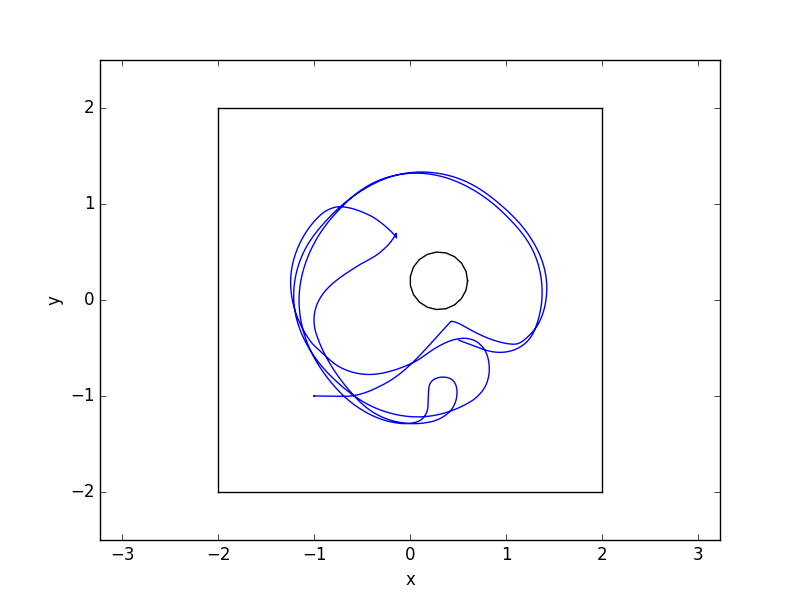
\includegraphics[width=\textwidth]{fig/2a.png}
			\caption{Braitenburg controller}
			\label{fig:braitenburg}
		\end{figure}

		\item The plot of the trajectory of the rule based controller is shown by figure \ref{fig:rule-based}. The basic idea is to slow down and eventually stop and reverse if the robot is about to hit an obstacle, rotating until there is a clear path. Otherwise, the robot will just go forward. There are 3 branches for different values of the front sensor. Less than 1, the speed increases linearly from -2m/s up to 1m/s, with it rotating until it can escape this branch (by finding a direction with no obstacles diredtly in front). Between 1 and 2, speed increases linearly again and the robot rotates, but slower.  Similarly, there are two branches for the front\_left and front\_right sensors for the case that there is an off centre obstacle that the front sensor doesn't detect. Similar to the braitenburg, the robot will attempt to rotate away from the obstacle depending on which sensor it is. If the robot is not close to an obstacle, it will just move forward with no rotation.
		\begin{figure}[h]
			\centering
			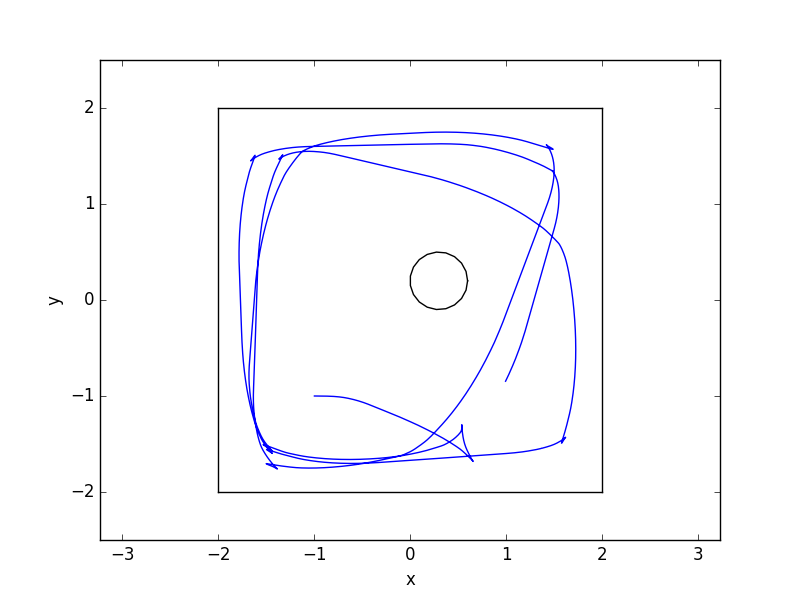
\includegraphics[width=\textwidth]{fig/2b.png}
			\caption{Rule-based controller}
			\label{fig:rule-based}
		\end{figure}

		\item 

        \item In the presence of no noise, the braitenburg controller is more robust, since it will never end up hitting an obstacle even in the presence of unexpected ones. The rule based controller will not 
\end{enumerate}
\section*{1.2 Localization}
\subsection*{Exercise 3}
\begin{enumerate}[label=(\alph*)]
	\item braitenburg
	\item My solution generates points uniformly inside the square, i.e. from -2 to 2 in both the x and y components. It also generates a random direction (from 0 to $2\pi$). It then checks to see whether the robots has been placed within the cylinder, and if it has, generates a new random pose. It continues until it returns a valid pose (which isnt inside the cylinder).
	\item The move function takes delta\_pose, which is an offset relative to the particle. From this, I take the x and y components and add a gaussian error with a standard deviation of 10\% of the magnitude of the movement. This x and y with the noise added is added to the pose of the particle. The same is done for the yaw component.
	\item The compute\_weight method calculated the new weight of a particle and updates it. If the particle moved outside the arena, then its weight is set to 0 so that it isn't sampled again. For the other particles, their weights are set to $ p(z|x) $, which is the probability of the measurement given the position of the particle. The measurement model is a normal centered around the measured value with a standard deviation of 80cm. The particles which are more likely to be in the correct postion are therefore given a higher weight, and so are much more likely to be resampled.
	\item e
	\item f
	\item g
	\item An extended Kalman Filter looks at landmarks as its measurement model, and only models gaussian measurement models. It is a lot more efficient - both in time and space complexity. It also needs to take an initial pose, whereas the particle filter does not.
\end{enumerate}




\end{document}
